\documentclass{article}
\usepackage{amsmath}
\usepackage{dcolumn}
\usepackage{threeparttable}
\usepackage{geometry}
\usepackage{graphicx}
\graphicspath{{../figures/}} % Specify the relatlive path to the "images" folder

\newcolumntype{d}[1]{D{.}{.}{#1}}

% Placeholder paragraphs with text
\usepackage{blindtext}

% No indent for new paragraphs
\setlength\parindent{0pt}

% bibliography
\usepackage[
    backend=biber,
    style=numeric,
    url=false,
    doi=false,
    eprint=false
]{biblatex}
\addbibresource{bibliography.bib}

% ---------------------------------------------------------------------------

\usepackage{graphicx}  % for including images
\usepackage{titling}   % for more control over the title
\title{\textbf{Analysis of Deposit Rate Pass Through Effects in Tightening Cycles}}

\author{Your Name}
\date{\today}
\geometry{top=2.5cm, bottom=2.5cm}
\begin{document}

\begin{titlepage}
    \centering
    \vspace*{-1.5cm} % Adjust the value as needed to reduce space
    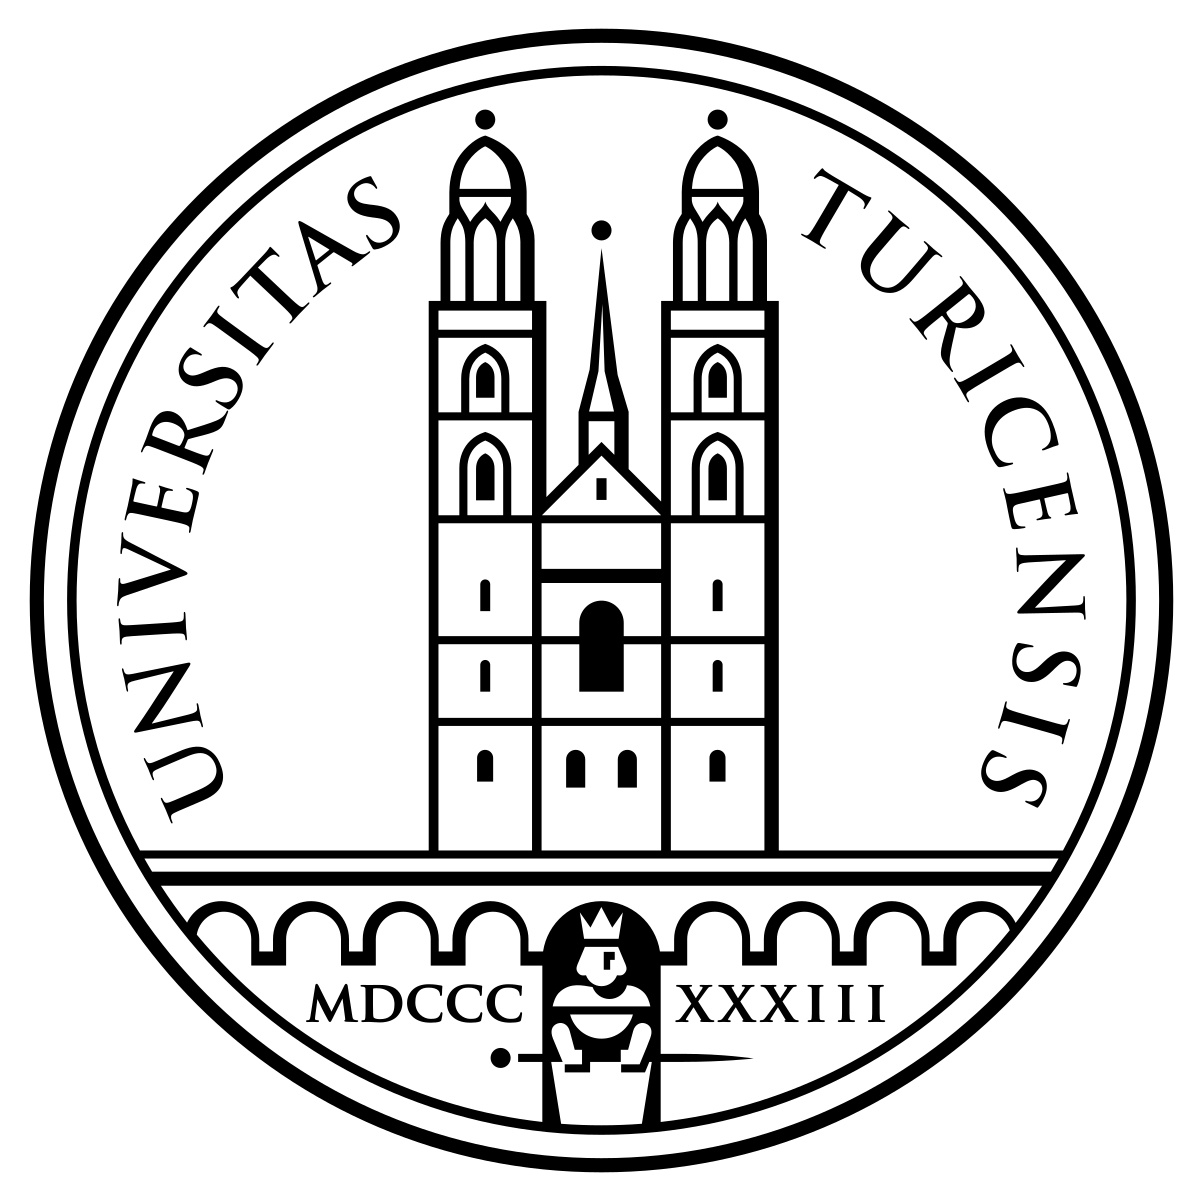
\includegraphics[width=0.4\textwidth]{figures/University_of_Zurich_seal.png} % Add your project logo
    
    \vspace{2cm}
    \Huge
    \textbf{Analysis of Deposit Rate Pass Through Effects in Tightening Cycles}
    
    \vspace{1cm}
    \LARGE
    This research project focuses on examining how savings deposit rates within a country respond to changes in central bank policy rates. 
    
    \vspace{1cm}
    \textbf{Authors:}\\ John Hojnacki \\ Matthew Aylward \\ Victoria Gemperle
    \vspace{1cm}
    
    \textbf{Date:}\\
    \thedate
    \vfill
    
\end{titlepage}


\section{Introduction}

    \linespread{1}  % Adjust the factor as needed
    
Central Banks around the world implement monetary policy in a variety of different ways, but one key transmission mechanism is typically a short-term rate at which commercial banks can borrow from the central bank. This rate, the ‘policy rate’, effectively becomes a floor on other rates, and measuring the sensitivity of other rates, such as the deposit rate, to changes in the policy rate, can give an indication as to how quickly monetary policy is transmitted in each cycle. For this project, the objective is to evaluate the sensitivity of deposit rates on consumer savings accounts to changes in the central banks’ policy rate across different economic cycles. Deposit rates are an important focal point because they affect the majority of households, and thus have a broad impact on society. The 2022 survey of Consumer Finance (US) found that 98.6\% of households had a transaction account, whereas only 11.5\% of households owned bonds\cite{scf2022}.\\

One way to measure the sensitivity of deposit rates to policy rates is by calculating the cumulative deposit beta, which measures the relative change in deposit rates to policy rates over the course of a hiking cycle. Researchers at the NY Federal Reserve have applied this analysis in a US Context and found that the most recent round of hiking may be on track to outpace previous cycles in terms of pass through effects\cite{deposit2023}. In this paper, we take inspiration from the research done on the US, and apply it to Switzerland, with some slight modifications to the method.

\section{Data}

This project requires only monthly policy rates and deposit rates for a particular country. If a country doesn't have a specific target, it may be extrapolated from a target range. In the example case, we use the midpoint of a range from the Swiss National Bank from 2000-2019, and then a target from 2019 onwards (they introduced a target at that time). If deposit rates are not available historically, or contain discrepancies due to changes in calculation methodology, as is the case in the US, alternative data may be employed with the same economic meaning. In the US case, the NY Fed utilizes bank financial reports to calculate the deposit rate as a function of interest paid on deposits over interest bearing deposits\cite{deposit2023}. The main criteria of the data used for this analysis is that it represents economically both the key policy rate of a central bank, and a key rate that is significant to consumers. Aside from this, creativity is encouraged.\\

\section{Methodology}

\subsection{Identification of Hiking Cycles}

The methodology for identifying hiking cycles utilizes a precise algorithm, with time (\( t \)) measured in monthly intervals. A hiking period is defined as a sequence of months during which there is a consistent increase in the policy rate. The criteria for a month to be considered part of a hiking period are as follows:

\begin{enumerate}
    \item \textbf{Direct Increase:} There must be an observed increase in the policy rate compared to the preceding month.
    
    \item \textbf{Look-Ahead Logic:} A month may also be considered part of a hiking period under the following condition:
    \begin{itemize}
        \item In cases where there is no month-over-month increase in the current period, but there was an increase in the previous period, and an increase is anticipated in the subsequent two months.
    \end{itemize}
\end{enumerate}

This forward-looking approach, termed 'look-ahead logic', is applicable in an ex-post analysis of historical data. The objective is not to predict future rate hikes but to classify them accurately within our dataset. By incorporating both immediate and anticipated policy rate movements, this methodology allows for a comprehensive and accurate identification of hiking periods.\\

\textbf{Inclusion Criteria and Unique Identifiers}

Critical to our analysis is the inclusion of the month preceding an official rate hike. Its inclusion is relevant to anchor the starting point and provide a basis for comparison as the hiking cycle progresses. Furthermore, each identified hiking period is assigned a unique identifier. This facilitates a granular analysis, allowing for a comparative assessment across different cycles.

\subsection{Calculation of Deposit Betas}

The deposit beta, (\( \beta_t \)), measures the magnitude of change in deposit rates relative to the change in policy rates, providing insights into the transmission mechanism of monetary policy.\\

The formula used for estimating deposit beta is:
\[
\beta_t = \frac{\Delta D_t}{\Delta P_t}
\]
where \( \Delta D_t \) represents the total change in deposit rates, and \( \Delta P_t \) denotes the total change in policy rates over the same period. The variable \( t \) signifies the time in months from the start of the hiking cycle. This calculation enables us to quantify the sensitivity of deposit rates to shifts in monetary policy.\\

\textbf{Interpretation of Results}

A higher value of \( \beta_t \) indicates a more pronounced response of deposit rates to changes in policy rates. By tracking the evolution of deposit beta from the onset of a hiking cycle to the peak of deposit rates, we gain an understanding of the lag and magnitude of the banking sector's response to central bank actions. This analysis is particularly pertinent in assessing the efficiency and impact of monetary policy.\\

The methodology applied in this project is designed to be replicable across different countries and time periods, which allows for its usage in scenarios where central banks provide explicit targets, target ranges, or operate without a clearly defined target. The project can be employed to analyze and compare the sensitivity of deposit rates on consumer savings accounts to changes in central banks’ policy rates across different economic and temporal contexts. This cross-country and cross-temporal applicability assures the project's utility in capturing variations in monetary policy transmission mechanisms globally.\\

\section{History in a Swiss Context}

\begin{figure}[h]
    \centering
    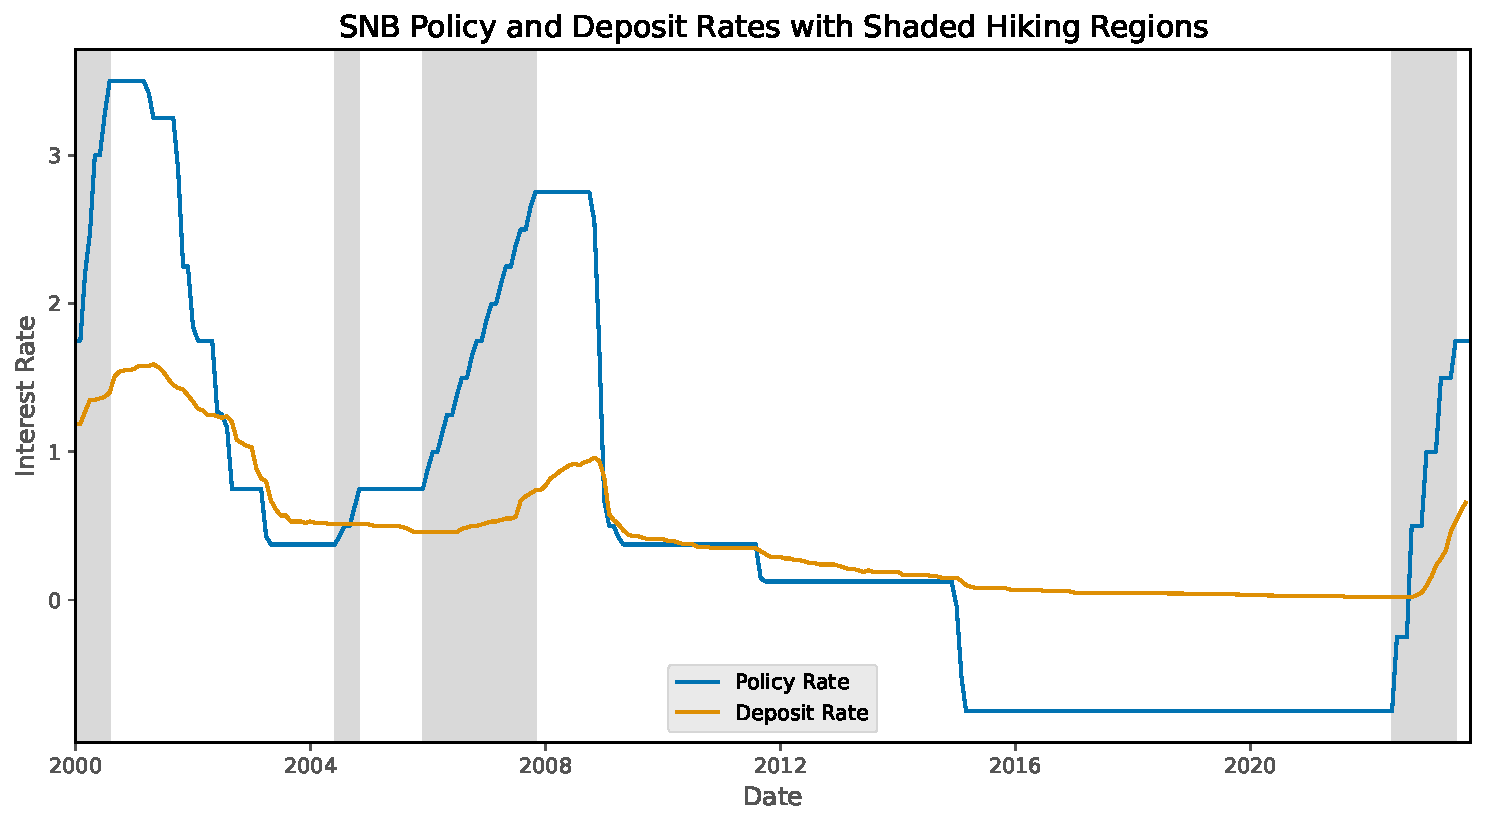
\includegraphics[width=1\textwidth]{Test/rates_shaded_SNB.pdf}
    \caption{Policy and Deposit Rates for Switzerland}
    \label{fig:rates_shaded}
\end{figure}

The above Figure 3 show the SNB target/target midpoint (pre-2019) vs. savings deposit rates. We have identified 4 cycles, from which 3 will be analysed. Some observations:

In December of 1999, the Swiss National Bank (‘SNB’) announced its intention to steer money market rates through the mechanism of a target range, a departure from the previous policy of targeting money supply. This change also coincided with the decision to begin tightening monetary policy over the next year. (source: SNB Quarterly bulletin, December 1999). This hiking cycle is the first of four which appears in the period of our analysis for Switzerland (2000, 2004, 4Q05-, and 2022-present day). However, the short hiking cycle in 2004 will be left out of our discussion for two reasons. First, the commentary from the SNB itself in the Monetary Policy Report at the time noted that while it was increasing the target range, overall policy remained expansionary. The second reason is that the hikes in this period were simply a reversal of the cuts which had taken place in March of 2003 to address deflation concerns. This resulted in no change in deposit rates, which interestingly had also experienced a muted reaction to the prior cut. The next true tightening of financial conditions began in March of 2006, and continued steadily until the Global Financial Crisis (“GFC”) necessitated easing of rates once again. The last hiking cycle begins in the wake of recovery from the Covid-19 Pandemic and continues through the time of this writing.\\ 


\begin{figure}[h]
    \centering
    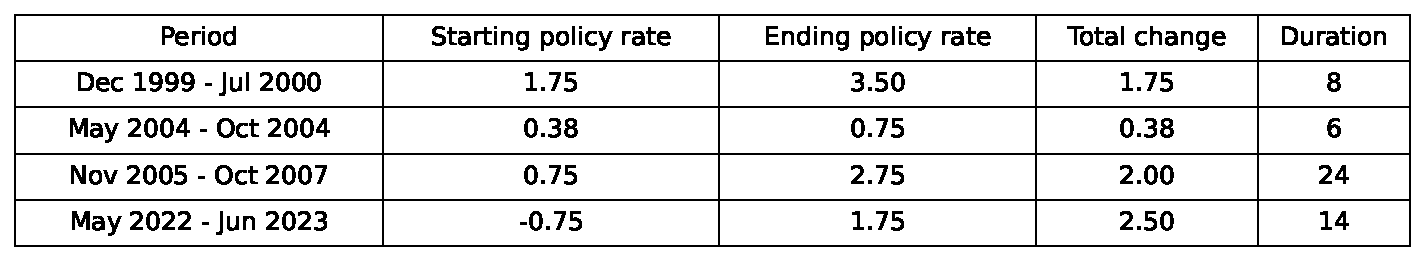
\includegraphics[width=1\textwidth]{Test/hiking_summary_SNB.pdf}
    \caption{Hiking Cycles Across Time}
    \label{fig:your_pdf}
\end{figure}

\begin{figure}[h]
    \centering
    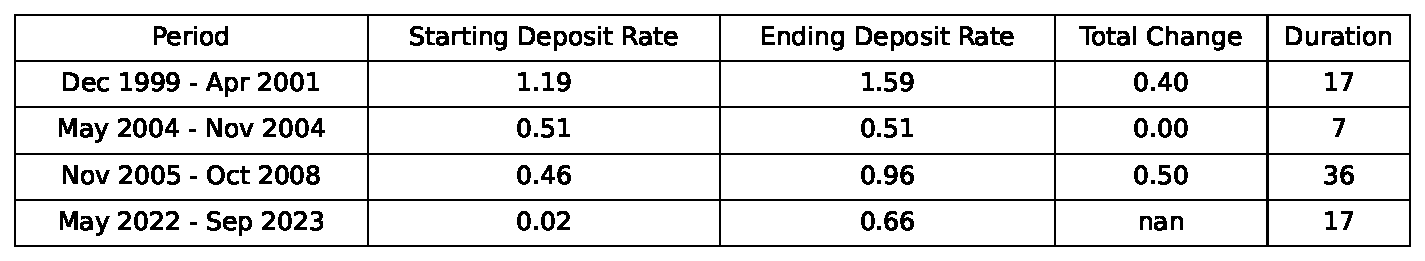
\includegraphics[width=1\textwidth]{Test/deposit_summary_SNB.pdf}
    \caption{Deposit Rates Summary across Hiking Periods}
    \label{fig:deposit_summary}
\end{figure}


The above Figure 1 and Figure 2 show the comparative statistics for current and previous rounds of hiking, for both Policy and Deposit Rates respectively. Some observations:

\begin{itemize}
    \item 2004 hikes were a reversal to a previous level, the policy remained "accommodating";
    \item Most recent cycle strongest from absolute and relative standpoint, but from zero starting point, this is not very informative in itself;
    \item We observe a 9 month lag to peak deposit in 2000, 12 month lag in 2005-2008. 
\end{itemize}

The observed trend indicates a noticeable lag effect, with the months to peak revealing a 9-month lag in the first two hikes and a 12-month lag in subsequent ones. According to the methodology, it is technically asserted that the policy hiking for the SNB has ended, as it has remained unchanged for a few months, and the deposit rate continues to achieve new highs. As of now, there is a recorded 2-month lag, and the duration of this lag is yet to be determined.
\\

\begin{itemize}
    \item The current cycle appears to demonstrate a higher degree of pass through in
terms of how quickly deposit rates began moving, and in how much of the
policy rate increases were being captured by the higher deposit rates;
    \item At a high level, there is a notable presence of a delay between the points in time when policy rates reach their peaks and when deposit rates reach their maximum levels.
\end{itemize}

\subsection{Deposit Betas}

For the deposit betas, a few observations:

\begin{itemize}
    \item Calculation: $\Delta$ deposit rate/$\Delta$ policy rate  (from beginning of each cycle);
    \item Deposit beta for current cycle (red) shows much quicker pass through effect than the ‘05-’08 hikes (blue). (Figure 4 below);
    \item Compared to ‘00 (grey), we’ve reached parity in total pass-through 5 quarters in, but the lagged effect likely to continue to increase;
    \item Insight: on-track for record deposit pass through. 
\end{itemize}

\begin{figure}[h]
    \centering
    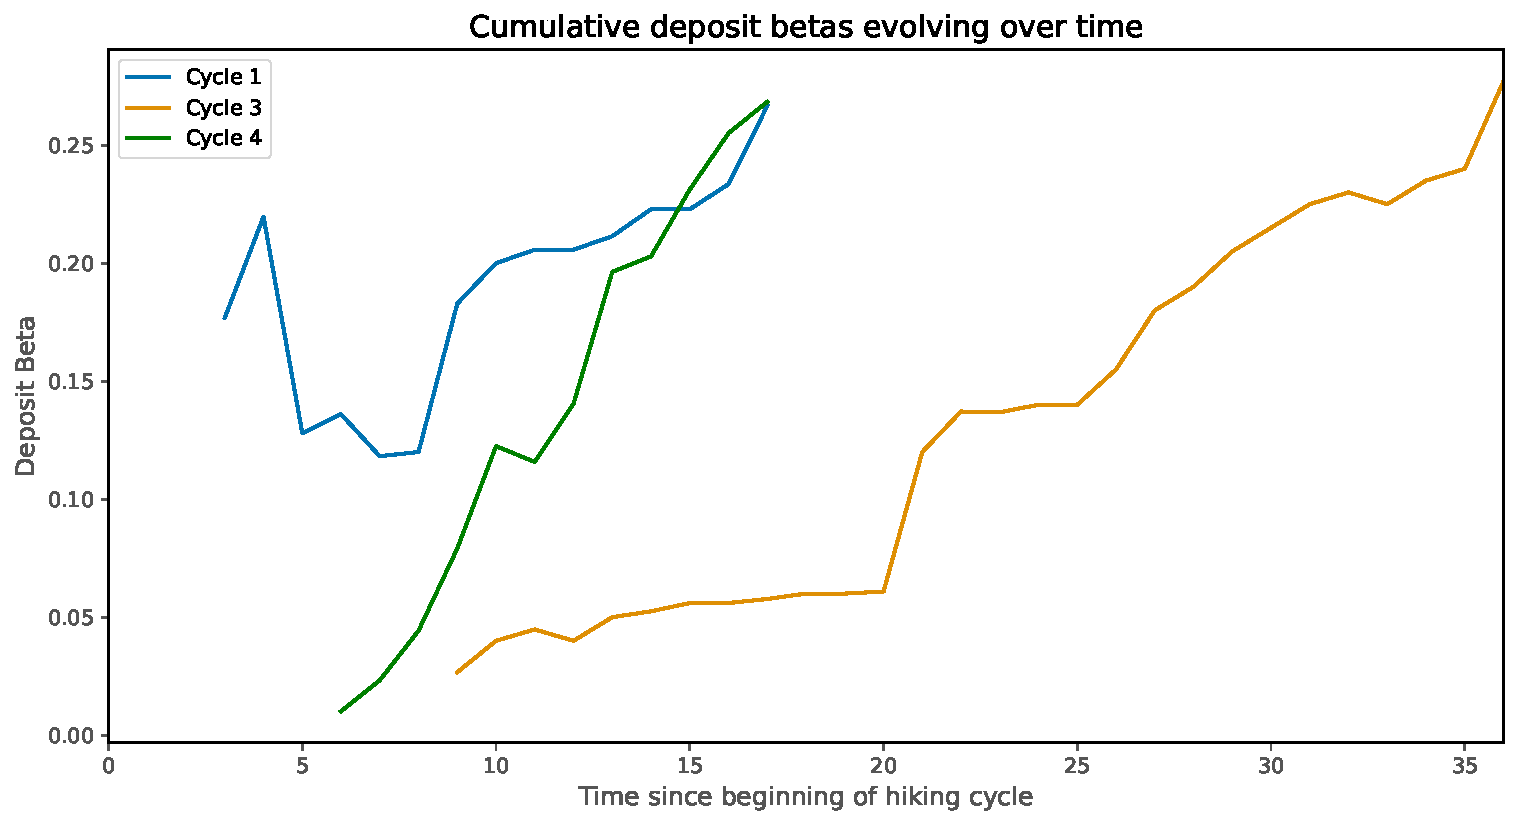
\includegraphics[width=1\textwidth]{Test/deposit_beta_SNB.pdf}
    \caption{Cumulative Swiss Deposit Betas in Hiking Cycles}
    \label{fig:your_pdf}
\end{figure}

The deposit beta is what confirms our intuition from the historical chart. It demonstrates that we are seeing much higher pass through (5 quarters in) vs. ‘05-08, and a comparable level of pass through to the 2000 hikes, but with only two months of lag so far. \\

For Switzerland, the answer to the research question is that in the current tightening cycle, deposit rates have moved much quicker, and will likely capture much more of the increase in policy rates than has happened in the last 25 years


% Bibliography section
\newpage  % Start a new page for the bibliography
\section{References}
\printbibliography[heading=none] 

\end{document}